\documentclass{article}

\usepackage{mathtools}
\usepackage{graphicx}
\usepackage{amsmath}
\usepackage{amsbsy}
\graphicspath{{images/}}

\begin{document}

\tableofcontents

\section{Equações químicas}
\subsection{Coeficientes e índices}

\section{Modelos atômicos}
\subsection{Dalton}
\subsection{Rutherford}
\subsection{Bohr}
\subsubsection{Postulados}
\subsubsection{Salto quântico}
\subsection{Schrödinger}
\subsection{Sommerfeld}
Veja \ref{modelo:sommerfeld}

\section{Partículas fundamentais}
\begin{itemize}
    \item Àtomo
    \begin{itemize}
        \item Núcleo
        \begin{itemize}
            \item Neutrons
            \item Prótons
        \end{itemize}

        \item Eletrosfera
        \begin{itemize}
            \item Níveis
            \item Elétrons
        \end{itemize}
    \end{itemize}
\end{itemize}
\subsection{Características}
\begin{tabular}{||c|c|c|c||}
    \hline
    Partícula & Carga & Massa & Representação \\
    \hline
    \hline
    Próton & $+1$ & $1u$ & $ \prescript{}{1}{p}^1 $ \\
    Nêutron & $0$ & $1u$ & $ \prescript{}{0}{n}^1 $ \\
    Próton & $+1$ & $1/1840u$ & $ \prescript{}{-1}{e}^0 $ \\
    \hline
    \hline
\end{tabular}
\begin{equation}
    \prescript{A}{Z}{X}^{\pm y}
\end{equation}
\begin{equation}
    N = A - Z
\end{equation}
\begin{equation}
    e^- = Z - y
\end{equation}
\begin{itemize}
    \item N° atômico \textbf{Z} $\rightarrow$ N° de prótons que o átomo possui
    \item N° de massa \textbf{A} $\rightarrow$ Soma dos prótons e nêutrons ($ A = Z + N $)
    \item N° de nêutrons \textbf{N} $\rightarrow$ ($ N = A - Z $)
    \item N° de elétrons \textbf{$ e^- $}
    \begin{itemize}
        \item Em átomos neutros $\rightarrow$ $ e = Z $
        \item Em cátions (+) $\rightarrow$ $ e = P - n $ onde $ n $ é igual a carga positiva do cátion
        \item Em ânions (-) $\rightarrow$ $ e = P - n $ onde $ n $ é igual a carga negativa do ânion
    \end{itemize}
\end{itemize}

\section{Relações atômicas}
\begin{itemize}
    \item Isóto\textbf{p}os: Mesmo número de prótons/número atômico (\textbf{P})
    \item Isób\textbf{a}ros: Mesmo número de massa (\textbf{A})
    \item Isóto\textbf{n}os: Mesmo número de nêutrons (\textbf{N})
    \item Iso\textbf{eletrôn}icos: Mesmo número de elétrons
\end{itemize}


\section{Organização da eletrosfera}
\subsection{Espectros de emissão}
\subsection{Modelo atômico de Sommerfeld} \label{modelo:sommerfeld}
Propões subníveis com base nos espectros de emissão que vão de \textbf{1} a \textbf{7} (veja tabela \ref{tabela:modelo_sommerfeld})
\begin{table}[h!]
    \centering
    \begin{tabular}{||c||c|c|c|c|c|c|c||}
        \hline
        \hline

        Nível & 1 & 2 & 3 & 4 & 5 & 6 & 7 \\
        & K & L & M & N & O & P & Q \\
        \hline

        Max elétrons & 2 & 8 & 18 & 32 & 32 & 18 & 8 \\
        \hline

        \hline
        \hline
    \end{tabular}

    \caption{Níves eletrônicos segundo Sommerfeld.}
    \label{tabela:modelo_sommerfeld}
\end{table}

Essas camadas, por sua vez, são dividadas em subníveis (veja tabela \ref{tabela:modelo_sommerfeld:subniveis})

\begin{table}[h!]
    \centering
    \begin{tabular}{||c||c|c|c|c|c|c|c||}
        \hline
        \hline

        Subnível & s & p & d & f \\
        \hline

        Elétrons & 2 & 6 & 10 & 14 \\
        \hline

        \hline
        \hline
    \end{tabular}

    \caption{Cada camada está dividida em subníveis, de acordo com o máximo de elétrons que ela suporta.}
    \label{tabela:modelo_sommerfeld:subniveis}
\end{table}

\section{Distribuição eletrônica}
\begin{center}
    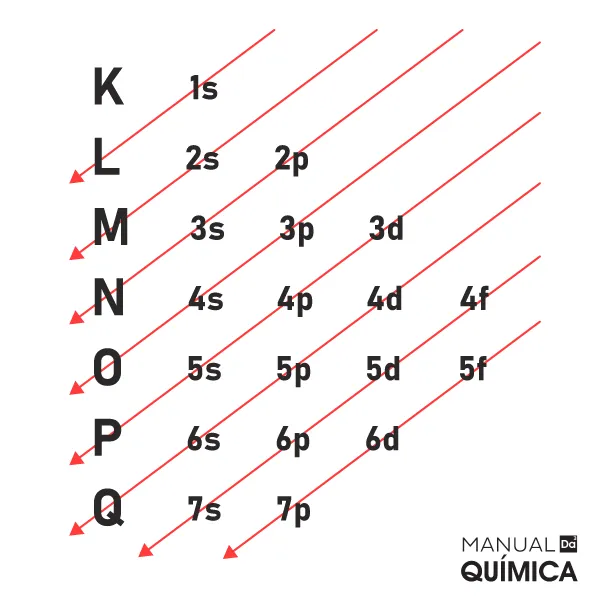
\includegraphics[width=0.875\textwidth]{distribuicao_eletronica}
\end{center}
\begin{equation}
    \prescript{}{26}{Fe} = 1s^2 2s^2 2p^6 3s^2 3p^6 \boldsymbol{4}s^2 \boldsymbol{3d^6}
\end{equation}

A \textbf{última \emph{camada}} (\textbf{4} no exemplo acima) é considerada a \emph{camada de valência} e o \textbf{último \emph{subnível}} (\textbf{$ 3p^6 $} no exemplo acima) é o \emph{subnível mais energético}.

\subsection{D. E. Cerne do gás nobre}
Utiliza a distribuição eletrônica de um gás nobre para simplificar.

\begin{equation}
    \prescript{}{16}{Ar} = 1s^2 2p^6 3s^2 3p^6
\end{equation}

\begin{equation}
    \prescript{}{26}{Fe} = [Ar]4s^2 3d^6
\end{equation}

\subsection{D. E. de íons}
Realiza a distribuição eletrônica com base no átomo neutro e retira (cátion) ou adiciona(ânion) a carga na camada de valência.

\begin{equation}
    \prescript{}{24}{Cr} = 1s^2 2s^2 2p^6 3s^2 3p^6 4s^2 3d^6
\end{equation}
\begin{equation}
    \prescript{}{24}{Cr}^{+3} = 1s^2 2s^2 2p^6 3s^2 3p^6 4s^2 3d^6
\end{equation}

\section{Tabela periódica}

\subsection{Evolução}
\begin{enumerate}
    \item Mendelev: Ordem crescente de \textbf{massas atômicas}
    \item Moseley: Ordem crescente de \textbf{números atômicos}
\end{enumerate}

\subsection{Organização}

\begin{itemize}
    \item \textbf{Lantanídeos} e \textbf{actinídeos } ficam \textbf{fora} da tabela.
    \item Períodos: 7 linhas \textbf{horizontais} em que os elementos possuem \textbf{o mesmo n° de níves energéticos}.
    \item Famílias
    \begin{itemize}
        \item \textbf{18 colunas}
        \item Agrupa elements de \textbf{propriedades semelhantes}
        \item EX: Família \textbf{1A} reage com água produzindo \boldmath{$ H_{2(g)} + {calor} $}
    \end{itemize}
\end{itemize}

\subsection{Classificação dos elementos}
\begin{itemize}
    \item Metais
    \item Ametais
    \item Semimetais
    \item Gases nobres
\end{itemize}

\begin{center}
    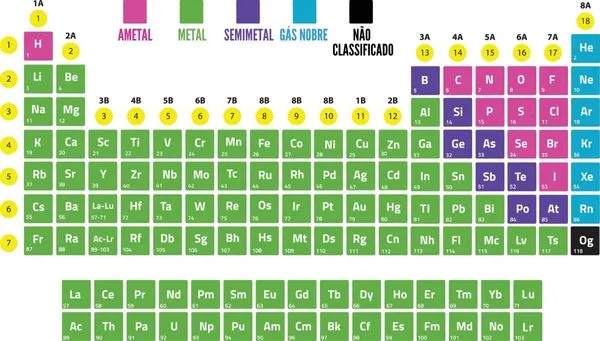
\includegraphics[width=1\textwidth]{tabela_periodica_categorias}
\end{center}

\subsection{Classificação de acordo com a distribuição eletrônica}

A Localização de um elemento na tablea se relaciona com a distribuição eletrônica:
\begin{itemize}
    \item A \textbf{camada de valência} indica o \textbf{período}
    \item O \textbf{subnível mais energético} indica a \textbf{família}
    \item obs: Lantanídeos e actinídeos sempre na família 3
\end{itemize}

\subsubsection{Divisões por subnível}
Elementos \textbf{representativos} são aqueles que possuem o subnível mais energético \textbf{s} ou \textbf{p}. Os elements de \textbf{transição} tem o seu subnível mais energético sendo \textbf{d} ou \textbf{p}, podendo ser de \textbf{transição externa} ou \textbf{transição interna}.
\begin{center}
    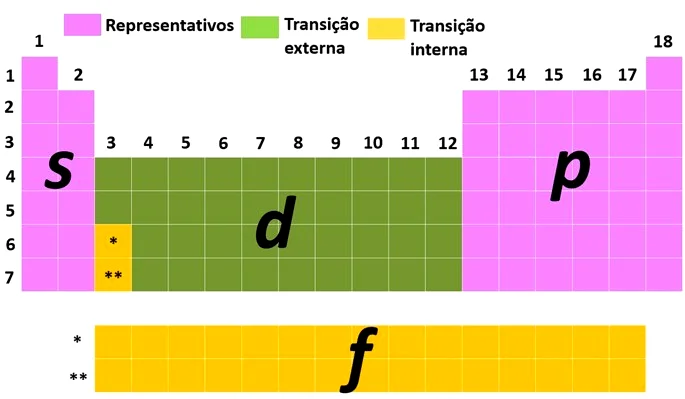
\includegraphics[width=1\textwidth]{tabela_periodica_divisoes_subnivel}
\end{center}

\subsection{Propriedades periódicas}
\subsubsection{Raio atômico}
O \textbf{raio atômico} é a \textbf{distância} entre dois núcleos de átomos vizinho de um mesmo elemento no estado sólido,
\textbf{aumentando} em uma mesma \textbf{família}, de \textbf{cima para baixo}, pois os elementos mais abaixo possuem mais camadas.
Já no período, \textbf{aumenta}, da \textbf{direita para a esquerda}, devido ao número de prótons.

Vale salientar que os \textbf{cátions} possuem raio atômico \textbf{menor} que o àtomo neutro, enquanto os \textbf{ânions} possuem um raio \textbf{maior}.

\begin{center}
    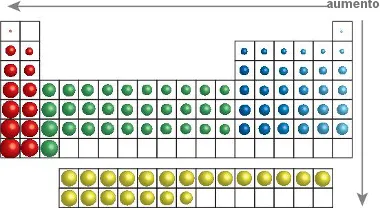
\includegraphics[width=1\textwidth]{tabela_periodica_raio_atomico}
\end{center}

\subsubsection{Periodicidade}
Uma valor menos um anterior é a um anterior menos aquele que vem antes.
EX: Considerando A, B, C e D números atômicos de elementos \textbf{ordenados} 
\begin{equation}
    C-B = B-A
\end{equation}

\subsubsection{Energia de ionização}
Energia necessária para \textbf{retirar um elétron} de um átomo \textbf{neutro} no estado \textbf{gasoso}, sendo mais fácil retirar o elétron que está mais longe do núcleo.

\begin{equation}
    X_{(g)} + E_i \rightarrow X^+_{(g)} + e^-
\end{equation}

\begin{center}
    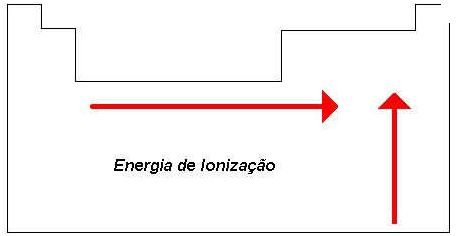
\includegraphics[width=1\textwidth]{tabela_periodica_energia_ionizacao}
\end{center}

\begin{itemize}
    \item \textbf{Inversamente proporcional} ao tamanho do átomo
    \item Quanto \textbf{mais elétrons} são \textbf{removidos}, mais \textbf{difícil} fica para se remover mais e vice-versa
    \item Um grande salto na $ E_i $ indica um salto de camada, saltos menores indicam saltos em subníveis
\end{itemize}

\subsection{Afinidade electrônica}
\textbf{Energia liberada} ao \textbf{adicionar um elétron} a um átomo \textbf{neutro} no estado \textbf{gasoso}.

\begin{equation}
    X_{(g)} + e^- \rightarrow X^-_{(g)} + E_{af}
\end{equation}

Pode ser considerada a \textbf{vontade de ter elétrons}.

Varia de forma contrária ao raio atômico.
\begin{itemize}
    \item Quanto \textbf{menor} o átomo, \textbf{maior} afinidade eletrônica
    \item \textbf{NÂO} se aplica a \textbf{gases nobres}
    \item O \textbf{flúor} é muito pequeno para receber elétrons por isso, o \textbf{cloro} tem a \textbf{maior afinidade eletrônica}
\end{itemize}

\begin{center}
    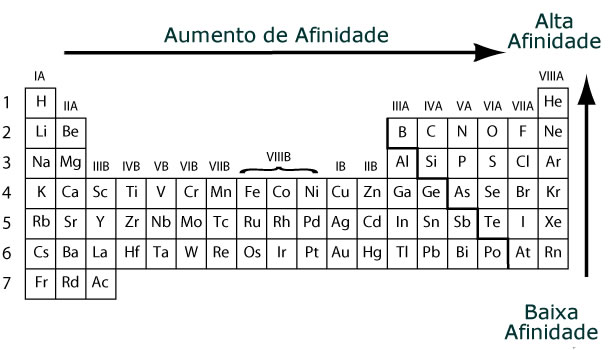
\includegraphics[width=1\textwidth]{tabela_periodica_afinidade_eletronica}
\end{center}

\subsection{Eletronegatividade}
\textbf{Força} com que um átomo \textbf{atrai} o par de elétrons de uma ligação, variando de forma \textbf{contrária} ao \textbf{raio atômico},
\textbf{não} sendo válido para a família dos \textbf{gases nobres}, já que não fazem ligação.
O elemento mais eletronegativo é o \textbf{flúor}.

\begin{equation}
    F > O > N \approx Cl > Br > I > S = C > P = H
\end{equation}

\begin{center}
    \textit{\textbf{FO}u\textbf{Cl}ore \textbf{Br}asileiro \textbf{I}ndio \textbf{S}em \textbf{C}ueca \textbf{P}elado \textbf{H}mmm..."}
\end{center}

\subsection{Densidade}
\begin{center}
    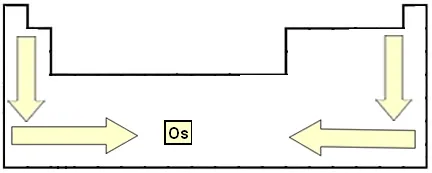
\includegraphics[width=1\textwidth]{tabela_periodica_densidade}
\end{center}

\subsection{Ponto de fusão e ponto de ebulição}
\begin{center}
    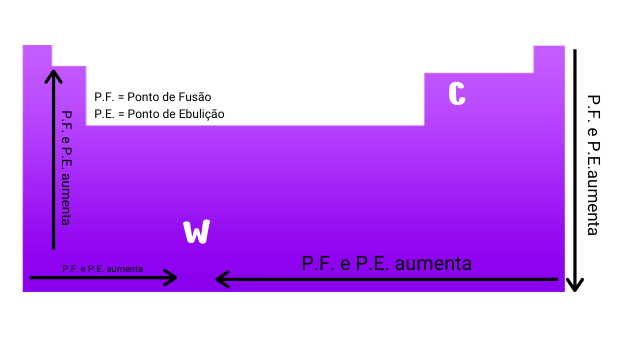
\includegraphics[width=1\textwidth]{tabela_periodica_p_fusao_p_ebulicao}
\end{center}

\subsection{Tabela unificada}
\begin{center}
    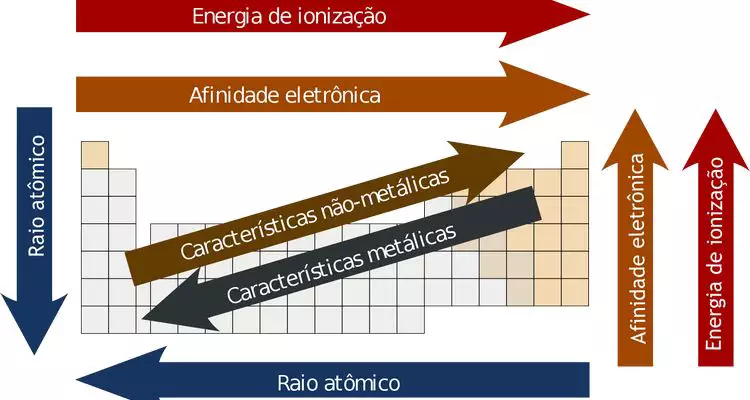
\includegraphics[width=1\textwidth]{tabela_periodica_unificada}
\end{center}

\section{Teoria do octeto}
\subsection{Regra do octeto}
Um átomo é \textbf{estável} quando possui \textbf{8 elétrons} em sua \textbf{camada de valência},
com \textbf{execeção} aqueles que possuem apenas \textbf{um nível} de energia, tornando-se estável com \textbf{2 elétrons},
pois é tudo o que cabe nessa camada.

\textbf{Metais} tendem a \textbf{perder} elétrons e \textbf{ametais} tendem a \textbf{ganhar} elétrons.


\section{Ligações}
\subsection{Ligação iônica}
Se dá pela \textbf{transferência de elétrons} de um átomo para outro,
que se mantém ligados pela \textbf{atração eletroestática}.
Possuem \textbf{altos pontos de fusão e ebulição}, devido a dificuldade de separar o
cátion do ânion e são \textbf{excelentes condutores de corrente elétrica} quando 
\textbf{fundidos} ou em \textbf{solução aquosa}.

\subsubsection{Formulação}
Sua formulação é baseada na \textbf{igualdade de cargas}

\begin{split}
    Na^+Cl^- \\ \text{\textit{obs: Após a ligação}}
\end{split}

Exemplos:
\begin{itemize}
    \item Para acontecer a ligação entre \boldmath{$ Ca^{2+} $} e \boldmath{$ PO_4^{3+} $},
        precisamos ajustar a quantidade de cada item para que as \textbf{cargas} sejam \textbf{iguais}: \boldmath{$ Ca_3(PO_4)_2 $}
    \item Para ligar \boldmath{$ Pb^4+ $} e \boldmath{$ SO_4^2- $} temos \boldmath{$ Pb(SO_4)_2 $}
\end{itemize}
\begin{equation}
    Ca^{2+} 
\end{equation}

\subsection{Ligação metálica}
Comumente chamada de \textbf{mar de elétrons}, pois os \textbf{cátions} ficam \textbf{fixos} e os \textbf{elétrons} se movem \textbf{livres}.

Algumas carascterísticas dos compostos metálicos são:
\begin{itemize}
    \item \textbf{Altos} pontos de \textbf{fusão} e \textbf{ebulição}, com algumas execeções;
    \item \textbf{Sólidos} a temperatura ambiente com exceção do mercúrio;
    \item \textbf{Bons} condutores \textbf{térmicos} e \textbf{elétricos};
    \item \textbf{Maleáveis}
    \item \textbf{Dúcteis}
\end{itemize}

As \textbf{ligas metálicas} sãos as \textbf{misturas} de metais, possuindo características próprias.

\subsection{Ligação covalente}
É uma ligação caracterizada pelo \textbf{compatilhamento de elétrons},
produzindo \textbf{compostos moleculares} com \textbf{baixos} pontos de fusão e ebulição,
podendo ser encontrados nos estados \textbf{sólidos,
líquidos e gasosos} em temperatura ambiente e \textbf{não conduzem corrente elétrica}.

É uma ligação que ocorre entre:
\begin{itemize}
    \item ametal + ametal
    \item ametal + hidrogênio
    \item hidrogênio + hidrogênio
\end{itemize}

\begin{itemize}
    \item Ligação covalente normal: \textbf{Cada} elétron do par vem de um átomo.
    \item Ligação covalente coordenada: \textbf{Ambos} os elétrons do par vem de um \textbf{mesmo átomo}
\end{itemize}

\subsection{Formulação}
\begin{enumerate}
    \item \textbf{Somar} os elétrons de \textbf{valência} de todos os átomos;
    \item Iniciando entre os \textbf{átomos ligantes}, realizar a \textbf{distribuição} dos elétrons nos \textbf{pares}
    \item De fora para dentro, \textbf{completar os octetos};
    \item Fazer rearranjos, se necessário.

\begin{center}
    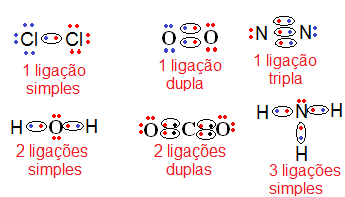
\includegraphics{ligacoes_covalentes}
\end{center}

\subsection{Íons poliatômicos}
Em \textbf{íons poliatômicos}, a carga não se encontra em um atómo em específico, mas sim,
\textbf{distribuída pelo íon}.

\end{enumerate}

\end{document}
